% !TeX spellcheck = ru_RU_yo
% !TEX program = xelatex

\documentclass[pta]{styles/scs-iam}

\begin{document}
  \pagestyle{headcenter}

  \newgeometry{
  top=20mm,
  right=15mm,
  bottom=20mm,
  left=20mm,
  bindingoffset=0cm
}

\thispagestyle{empty}

\begin{center}
  {
    \bfseries
    {
      \subnormal
      Министерство науки и высшего образования Российской Федерации
    } \\[-0.5em]
    {
      \scriptsize
      ФЕДЕРАЛЬНОЕ ГОСУДАРСТВЕННОЕ АВТОНОМНОЕ ОБРАЗОВАТЕЛЬНОЕ УЧРЕЖДЕНИЕ ВЫСШЕГО ОБРАЗОВАНИЯ
    } \\[-0.25em]
    {
      \subnormal
      “САНКТ-ПЕТЕРБУРГСКИЙ НАЦИОНАЛЬНЫЙ ИССЛЕДОВАТЕЛЬСКИЙ \\[-0.5em]
      УНИВЕРСИТЕТ ИНФОРМАЦИОННЫХ ТЕХНОЛОГИЙ, \\[-0.75em]
      МЕХАНИКИ И ОПТИКИ”
    } \\[3.25em]
    {
      \normalsize
      ВЫПУСКНАЯ КВАЛИФИКАЦИОННАЯ РАБОТA
    } \\[3.25em]
    {
      \normalsize
      <<РАЗРАБОТКА СИСТЕМЫ СБОРКИ \\[-0.5em]
      EMBEDDED LINUX>>
    } \\[5.75em]
  }
\end{center}

\begin{flushright}
  {
    \small
    \begin{minipage}{.7\textwidth}
      \titledline{Автор}\addsignatureskip
      \hspace{-5pt}$\underset{\text{\scriptsize (Фамилия, Имя, Отчество)}}{\underline{\makebox[\remaining][s]{\strut\hfill Яшин Александр Павлович\hfill}}}$
      \hfill
      \signature \\[-0.5em]

      \titledline{Направление подготовки (специальность)}
      $\underset{\text{\scriptsize (код, наименование)}}{\underline{\makebox[\remaining][s]{\strut\hfill 09.03.01 --\hfill}}}$ \\[-0.5em]
      $\underline{\makebox[\textwidth][s]{\strut\hfill Информатика и вычислительная техника\hfill}}$ \\[-0.5em]

      \titledline{Квалификация}
      $\underset{\text{\scriptsize (бакалавр, магистр)}}{\underline{\makebox[\remaining][s]{\strut\hfill бакалавр\hfill}}}$ \\[-0.5em]

      \titledline{Руководитель ВКР}\addsignatureskip
      \hspace{-5pt}$\underset{\text{\scriptsize (Фамилия, И., О.,  ученое звание, степень)}}{\underline{\makebox[\remaining][s]{\strut\hfill Ключев А. О., к.т.н. доцент\hfill}}}$
      \hfill\signature \\[3em]

      \textbf{К защите допустить} \\[0.25em]
      \titledline{Руководитель ОП}\addsignatureskip
      \hspace{-5pt}$\underset{\text{(Фамилия, И., О.,  ученое звание, степень)}}{\underline{\makebox[\remaining][s]{\strut\hfill Алиев Т.И., д.т.н, профессор\hfill}}}$
      \hfill\signature \\[-0.25em]

      \hfill\datetemplatealiev
    \end{minipage}
  }
\end{flushright}

\vfill

\begin{center}
  {
    \normalsize
    Санкт-Петербург, 2019 г.
  }
\end{center}

\restoregeometry

\clearpage

\newgeometry{
  top=20mm,
  right=20mm,
  bottom=20mm,
  left=15mm,
  bindingoffset=0cm
}

\thispagestyle{empty}

{
  \small
  \parindent0pt

  Студент
  $\underset{\text{\scriptsize (Фамилия, Имя, Отчество)}}{\underline{\text{\strut ~Яшин Александр Павлович~}}}$
  \hfill
  Группа
  $\underline{\text{\strut ~P3402~}}$
  \hfill
  Факультет
  $\underline{\text{\strut ~ПИиКТ~}}$ \\[-0.5em]

  \titledline{Направленность (профиль), специализация}
  $\underline{\makebox[\remaining][s]{\strut\hfill 09.03.01 --\hfill}}$
  $\underline{\makebox[\textwidth][s]{\strut\hfill Вычислительные машины, комплексы, системы и сети \hfill}}$ \\[0.25em]

  ВКР принята \datetemplate \\[-1em]

  Оригинальность ВКР $\underline{\makebox[7em][s]{\strut}}$\,\% \\[-1em]

  ВКР выполнена с оценкой $\underline{\makebox[12em][s]{\strut}}$ \\[-1em]

  Дата защиты \datetemplate \\[-1em]

  \titledline{Секретарь ГЭК}\addsignatureskip
  \hspace{-5pt}$\underset{\text{\scriptsize (Фамилия, И., О.)}}{\underline{\makebox[\remaining][s]{\strut}}}$
  \hfill\signature \\[0.25em]

  Листов хранения $\underline{\makebox[12em][s]{\strut}}$ \\[-1em]

  Демонстрационных материалов/Чертежей хранения $\underline{\makebox[12em][s]{\strut}}$
}

\restoregeometry

\clearpage

  \newgeometry{
  top=20mm,
  right=15mm,
  bottom=20mm,
  left=20mm,
  bindingoffset=0cm
}

\thispagestyle{empty}

\begin{center}
  {
    \bfseries
    {
      \subnormal
      Министерство образования и науки Российской Федерации
    } \\[-0.5em]
    {
      \scriptsize
      ФЕДЕРАЛЬНОЕ ГОСУДАРСТВЕННОЕ АВТОНОМНОЕ ОБРАЗОВАТЕЛЬНОЕ УЧРЕЖДЕНИЕ ВЫСШЕГО ОБРАЗОВАНИЯ
    } \\[-0.25em]
    {
      \subnormal
      “САНКТ-ПЕТЕРБУРГСКИЙ НАЦИОНАЛЬНЫЙ ИССЛЕДОВАТЕЛЬСКИЙ \\[-0.5em]
      УНИВЕРСИТЕТ ИНФОРМАЦИОННЫХ ТЕХНОЛОГИЙ, \\[-0.75em]
      МЕХАНИКИ И ОПТИКИ” \\[2em]
    }
  }
\end{center}

\small

\begin{flushright}
  \begin{minipage}{.5\textwidth}
    {
      \hfill\textbf{УТВЕРЖДАЮ}\hfill
    }

    \titledline{Руководитель ОП}

    \setlength{\remaining}{\textwidth}\addsignatureskip
    $\underset{\text{\scriptsize (Фамилия, И.О.)}}{\underline{\makebox[\remaining][s]{\strut\hfill}}}$
    \hfill\signature \\[-0.5em]

    \hfill\datetemplate \\[0.35em]
  \end{minipage}
\end{flushright}

\begin{center}
  {
    \bfseries
    {
      \normalsize
      З А Д А Н И Е \\
    }
    НА  ВЫПУСКНУЮ  КВАЛИФИКАЦИОННУЮ  РАБОТУ \\[1.5em]
  }
\end{center}

{
  \parindent0pt

  \textbf{Студенту}
  $\underline{\text{\strut Яшину А.П.~~}}$
  \hfill
  \textbf{Группа}
  $\underline{\text{\strut P3402~~}}$
  \hfill
  \textbf{Факультет}
  $\underline{\text{\strut ПИиКТ~~}}$ \\[-0.5em]

  \titledline{\textbf{Руководитель ВКР}}
  $\underset{
    \text{\scriptsize (ФИО, ученое звание, степень, место работы, должность)}
  }{
    \underline{\makebox[\remaining][s]{\strut Ключев Аркадий Олегович, к.т.н., доцент Университет ИТМО\hfill}}
  }$ \\[-0.5em]

  \textbf{1 Наименование темы}
  \uline{Разработка системы сборки Embedded Linux\hfill} \\[-1em]
  
  \titledline{\textbf{Направление подготовки (специальность)}}
  $\underline{
    \makebox[\remaining][s]{\strut 09.03.01 -- Информатика и вычислительная техника\hfill}
  }$ \\[-1em]

  \titledline{\textbf{Направленность (профиль)}}
  $\underline{
    \makebox[\remaining][s]{\strut Вычислительные машины, комплексы, системы и сети\hfill}
  }$ \\[-1em]

  \titledline{\textbf{Квалификация}}
  $\underline{
    \makebox[\remaining][s]{\strut бакалавр\hfill}
  }$ \\[-1em]

  \textbf{2 Срок сдачи студентом законченной работы}\hfill\datetemplate \\[-1em]

  \textbf{3 Техническое задание и исходные данные к работе} \\
  \uline{
    Изучить специфику работы встраиваемых устройств на основе Linux, провести обзор существую-\hfill
  }\\
  \uline{
    щих решений, реализующих сборку Linux для встраиваемых устройств, провести сравнение.\hfill
  }\\
  \uline{
    Разработать систему сборки Embedded Linux, провести тестирование и апробацию.\hfill
  }\\
  \uline{
    Требования к системе сборки:\hfill
  }\\
  \uline{
    - Кроссплатформенность;\hfill
  }\\
  \uline{
    - Возможность вручную конфигурировать необходимые предустановленные в образ пакеты;\hfill
  }\\
  \uline{
    - Возможность одновременной сборки нескольких образов: минимального, серверного, расширен-\hfill
  }\\
  \uline{
    ного;\hfill
  }\\[-1em]
}

\restoregeometry

\clearpage

\newgeometry{
  top=20mm,
  right=20mm,
  bottom=20mm,
  left=15mm,
  bindingoffset=0cm
}

\thispagestyle{empty}

{
  \parindent0pt

  \textbf{4 Содержание выпускной квалификационной работы (перечень подлежащих разработке вопросов)} \\
  \uline{
    4.1 Анализ предметной области;\hfill
  }\\
  \uline{
    4.2 Обзор существующих решений, реализующих сборку Linux для встраиваемых устройств;\hfill
  }\\
  \uline{
    4.3 Описание процесса проектирования, разработки и тестирования системы сборки;\hfill
  }\\
  \uline{
    4.4 Апробация результатов разработки.\hfill
  }\\[-1em]

  \textbf{5 Перечень графического материала (с указанием обязательного материала)} \\
  \uline{
    Презентация по проделанной работе (в формате PDF)\hfill
  }\\  
  \uline{
    Слайды:\hfill
  }\\ 
  \uline{
    - "Постановка задачи"\hfill
  }\\  
  \uline{
    - "Обзор существующих решений"\hfill
  }\\
  \uline{
    - "Примеры результатов работы системы"\hfill
  }\\[-1em]

  \textbf{6 Исходные материалы и пособия} \\
  \uline{
    6.1 Аппаратные и программные средства встраиваемых систем [Электронный ресурс]: учебное пособие/ А.О. Ключев [и др.].— Электрон. текстовые данные.— СПб.: Университет ИТМО, 2010.— 291 c.— Режим доступа: https://books.ifmo.ru/file/pdf/686.pdf \hfill
  }\\
  \uline{
    6.2 Yocto Project Mega-Manual [Электронный ресурс] // Linux Foundation. - 2010-2019. - Режим доступа: https://www.yoctoproject.org/docs/current/mega-manual/mega-manual.html\hfill
  }\\
  \uline{
    6.3 Armbian Documentation [Электронный ресурс] // Armbian. - 2019. - Режим доступа: https://docs.a\hfill
  }\\
  \uline{
    rmbian.com\hfill
  }\\
  \uline{
   6.4 The Buildroot user manual [Электронный ресурс] // Buildroot Association. - 2019 - Режим доступа: https://buildroot.org/downloads/manual/manual.html\hfill
  }\\[-1em]

  \textbf{7 Дата выдачи задания} \datetemplate\\[-1em]

  Руководитель ВКР~~\signature\\[-1em]

  Задание принял к исполнению~~\signature\hfill\datetemplate\\
}

\normalsize
\restoregeometry

\clearpage

  \newgeometry{
  top=20mm,
  right=15mm,
  bottom=20mm,
  left=20mm,
  bindingoffset=0cm
}

\thispagestyle{empty}

\begin{center}
  {
    \bfseries
    {
      \subnormal
      Министерство образования и науки Российской Федерации
    } \\[-0.5em]
    {
      \scriptsize
      ФЕДЕРАЛЬНОЕ ГОСУДАРСТВЕННОЕ АВТОНОМНОЕ ОБРАЗОВАТЕЛЬНОЕ УЧРЕЖДЕНИЕ ВЫСШЕГО ОБРАЗОВАНИЯ
    } \\[-0.25em]
    {
      \subnormal
      “САНКТ-ПЕТЕРБУРГСКИЙ НАЦИОНАЛЬНЫЙ ИССЛЕДОВАТЕЛЬСКИЙ \\[-0.5em]
      УНИВЕРСИТЕТ ИНФОРМАЦИОННЫХ ТЕХНОЛОГИЙ, \\[-0.75em]
      МЕХАНИКИ И ОПТИКИ”
    }
  }
\end{center}

\small

\begin{center}
  \vskip -1em
  {
    \bfseries
    {
      \large
      АННОТАЦИЯ \\
    }
    ВЫПУСКНОЙ  КВАЛИФИКАЦИОННОЙ  РАБОТЫ \\[1.5em]
  }
\end{center}

{
  \parindent0pt

  \titledline{\textbf{Студент}}
  $\underset{
    \text{\scriptsize (Фамилия, Имя, Отчество)}
  }{
    \underline{\makebox[\remaining][s]{~Яшин Александр Павлович\hfill}}
  }$ \\[-0.5em]

  \textbf{Наименование темы ВКР}
  \uline{~Разработка системы сборки Embedded Linux \hfill} \\[-1em]

  \textbf{Наименование организации, где выполнена ВКР}
  \uline{~Университет ИТМО\hfill} \\[-1.75em]
}

\begin{center}
  \textbf{ХАРАКТЕРИСТИКА ВЫПУСКНОЙ КВАЛИФИКАЦИОННОЙ РАБОТЫ}
\end{center}

\vskip -1em

{
  \parindent0pt

  \textbf{1 Цель исследования}
  \uline{Создание веб-приложения для обеспечения взаимодействия пользователя с~программным пакетом RTKLIB, используемым во~встраиваемом решении, с~помощью кроссплат\-форменного графического интерфейса\hfill} \\[-1em]

  \textbf{2 Задачи, решаемые в ВКР} \\
  \uline{
    2.1 Изучение состава и~возможностей программного комплекса RTKLIB;\hfill
  }\\
  \uline{
    2.2 Анализ существующих веб-приложений, предназначенных для работы устройствами, у~кото\-рых отсутствую органы управления;\hfill
  }\\
  \uline{
    2.3 Проектирование и~разработка приложения;\hfill
  }\\
  \uline{
    2.4 Тестирование и~апробация разработанного приложения.\hfill
  }\\[-1em]

  \textbf{3 Число источников, использованных при составлении обзора}
  \uline{\hfill 8\hfill} \\[-1em]

  \textbf{4 Полное число источников, использованных в работе}
  \uline{\hfill 38\hfill} \\[-1em]

  \textbf{5 В том числе источников по годам}
  \begin{figure}[h!]
    \centering
    \begin{tabular}{| *{6}{>{\centering\small\vspace{2pt}}m{2cm} |}}
      \toprule
      \multicolumn{3}{|>{\bfseries\small}c|}{Отечественных} & \multicolumn{3}{>{\bfseries\small}c|}{Иностранных} \tabularnewline
      \midrule
      Последние 5 лет & От 5 до 10 лет & Более 10 лет & Последние 5 лет & От 5 до 10 лет & Более 10 лет \tabularnewline
      \midrule
      7 & 0 & 0 & 31 & 0 & 0 \tabularnewline
      \bottomrule
    \end{tabular}
  \end{figure}\\[-2.5em]

  \titledline{\textbf{6 Использование информационных ресурсов Internet}}
  $\underset{
    \text{(да, нет, число ссылок в списке литературы)}
  }{
    \underline{\makebox[\remaining][s]{\hfill да, 37 \hfill}}
  }$
}

\restoregeometry

\clearpage

\newgeometry{
  top=20mm,
  right=20mm,
  bottom=20mm,
  left=15mm,
  bindingoffset=0cm
}

\thispagestyle{empty}

{
  \parindent 0pt

  \textbf{7 Использование современных пакетов компьютерных программ и технологий}
  \begin{figure}[h!]
    \centering
    \begin{tabular}{| >{\small\vspace{2pt}}m{10cm} | >{\centering\small\vspace{2pt}}m{3cm} |}
      \toprule
      \centering\textbf{Пакеты компьютерных программ и технологий} & \textbf{Раздел работы} \tabularnewline
      \midrule
      Программный пакет RTKLIB & 1, 2, 3, 4 \tabularnewline
      \midrule
      Язык программирования JavaScript & 3 \tabularnewline
      \midrule
      Менеджер пакетов NPM (Node.js) & 3 \tabularnewline
      \midrule
      Система сборки веб-приложений Webpack & 3 \tabularnewline
      \midrule
      Babel (транспилер) & 3 \tabularnewline
      \bottomrule
    \end{tabular}
  \end{figure}\\[-2.5em]

  \textbf{8 Краткая характеристика полученных результатов}
  \uline{В~результате работы было разработано веб-приложение, позволяющее пользователю взаимодействовать с~программным пакетом RTKLIB, используемым в~ГНСС-модулях и~ГНСС-приёмниках компании Emlid. Разработанное приложение было протестировано и~успешно прошло апробацию у~пользователей.\hfill} \\[-1em]

  \titledline{\textbf{9 Полученные гранты, при выполнении работы}}
  $\underset{
    \text{(название гранта)}
  }{
    \underline{\makebox[\remaining][s]{\hfill нет\hfill}}
  }$ \\[-1em]

  \titledline{\textbf{10 Наличие публикаций и выступлений на конференциях по теме выпускной работы}}
  $\underset{
    \text{(да, нет)}
  }{
    \underline{\makebox[\remaining][s]{\hfill да\hfill}}
  }$ \\[0.5em]
  \titledline{а) 1}
  $\underset{
    \text{(Библиографическое описание публикаций)}
  }{
    \underline{\makebox[\remaining][s]{\hfill}}
  }$ \\[0.5em]
  \titledline{б) 1}
  $\underset{
    \text{(Библиографическое описание выступлений на конференциях)}
  }{
    \underline{\makebox[\remaining][s]{Кузнецов А.А. Разработка веб-приложения для работы с программным пакетом высокоточно-}}
  }$
  \uline{го позиционирования RTKLIB // Конференция: XLVII Научная и учебно-методическая конферен\-ция Университета ИТМО, секция: Итоги выполнения НИР с участием магистрантов и аспирантов, подсекция: Исследование и разработка в области информационных технологий, 2018.\hfill} \\[-3em]
  \begin{flushright}
    2~\,\underline{\makebox[\remaining][s]{Кузнецов А.А. Разработка веб-приложения для работы с программным пакетом высокоточно-}}
  \end{flushright}
  \vskip -0.75em
  \uline{го позиционирования RTKLIB // Конференция: VII Конгресс молодых учёных, секция: Информа\-ционные технологии, 2018.\hfill} \\[-1em]

  Студент
  $\underset{
    \text{\scriptsize (Фамилия, И., О.)}
  }{
    \underline{\makebox[12em][s]{\strut\hfill}}
  }$~~ \signature\\[-0.5em]
  
  Руководитель
  $\underset{
    \text{\scriptsize (Фамилия, И., О.)}
  }{
    \underline{\makebox[12em][s]{\strut\hfill}}
  }$~~ \signature\\[-0.5em]
  
  \datetemplate
}

\normalsize
\restoregeometry

\clearpage


  \setcounter{page}{4}

  \section*{СОДЕРЖАНИЕ}
  \tableofcontents

  \newpage

  \mysection*{ВВЕДЕНИЕ}

\textbf{Актуальность темы}. В~настоящее время встраиваемые системы используются во сногих сферах человеческой деятельности. С помощью встраиваемых систем множество сложных процессов способны осуществляться легко, безопасно, вовремя, точно и непрерывно. Такие системы вносят серьезные изменения в повседневную жизнь людей.

Ядро Linux может работать на разных компьютерных архитектурах, большинство из которых довольно популярны во встроенном мире. Все базовые пакеты, позволяющие ОС выполнять основные задачи, подходят для кросс-компиляции, поэтому Linux может быть таким же распространенным, как микроконтроллеры и системы на кристалле (SoC).

\textbf{Цель работы.} Целью данного дипломного проекта является проектирование и реализация системы сборки Linux дистрибутивов для встроенных систем.

\textbf{Задачи работы.} Для достижения поставленной цели необходимо решить следующие задачи:

\begin{dashitemize}
  \item провести анализ существующих систем сборки 
  \item определить требования к системе сборки 
  \item спроектировать архитектуру системы сборки 
  \item реализовать программное обеспечение системы сборки в соответствии с разработанной архитектурой 
  \item произвести тестирование и апробацию
\end{dashitemize}

\textbf{Апробация результатов работы}. Наличие документации позволило осуществить открытое тестирование приложения пользователями и, как результат, получить отзывы, сообщения об ошибках и пожелания к функциональности.


Объем и структура работы. 
Работа содержит 999 страниц печатного текста, 999 рисунков, 999 таблицы, список литературы, включающий 999 источников. 
Работа состоит из введения, четырех частей и заключения. 
Во введении обоснована актуальность работы, определены цель и задачи исследования. 
В первой части произведено краткое описание встроенных систем, а также анализ существующих решений, реализующих сборку Linux дистрибутивов. 
Вторая часть содержит описание процесса проектирования архитектуры системы сборки. 
Третья глава описывает реализацию программного обеспечения. 
Четвертая глава описывает тестирование реализованного программного обеспечения. 
В заключении приведены основные результаты работы и возможные направления для дальнейшего развития.
\newpage

  % \mysection{АНАЛИЗ ПРЕДМЕТНОЙ ОБЛАСТИ}
\subsection{Встроенные системы}
\label{subsec:linux-for-embedded-systems}

\textbf{Встроенные вычислительные системы} (ВВС) – специализированные (заказные) вычислительные системы (ВС), непосредственно взаимодействующие с объектом контроля или управления и объединенные с ним единой конструкцией \cite{EMBEDDED}.

В силу специфики использования, обычно встроенные системы имеют низкое энергопотребление, предназначены для выполнения определенного набора задач и не являются универсальной вычислительной платформой, такой как компьютеры. По этим причинам, многие встроенные системы не используют операционную систему. Тогда программист проводит собственную разработку всего программного обеспечения, которое управляет оборудованием, практически не задействовав многозадачность и взаимодействие с пользователем. Программное обеспечение в таком случае работает непосредственно с оборудованием встроенной системы.

Однако в современном мире существуют более сложные встроенные системы, с расширенным списком решаемых задач. 
В такой многозадачной системе, должны быть реализованы следующие механизмы:
\begin{itemize}
  \item распределение памяти;
  \item предоставление времени ЦП разным потокам, процессам;
\end{itemize}

В таком случае программист может использвать ОС, это подход позволяет сосредоточиться на решении задачи, возложенной на ВВС, делегировав управление аппаратными средствами ОС.

Однако операционные системы очень трудно создавать, и это приводит к увеличению количества строк кода в проекте. 
При этом важно отметить, что влияние на количество ошибок в коде оказывает количество строк, то есть чем больше строк, тем больше ошибок \cite{EMBEDDED}. 
По этой же причине уст­ра­не­ние всех оши­бок в прак­ти­че­ски зна­чи­мом ПО слиш­ком тру­до­ём­ко, вме­сто это­го при его соз­да­нии обыч­но пы­та­ют­ся дос­тичь мак­си­маль­но воз­мож­но­го при за­дан­ных за­тра­тах уров­ня ка­че­ст­ва, как мож­но боль­ше сни­зить ве­ро­ят­ность про­яв­ле­ния оши­бок и ущер­ба от них. 
Так как операционные системы развиваются и поддерживаются в течение долгого периода времени\cite{TANENBAUM}, то во встроенных решениях часто используют уже существующие ОС.

\newpage
\subsection{Linux во встроенных системах}

Большое распространение во встроенных системах получили ОС на основе Linux.

\textbf{Дистрибутив Linux} - это операционная система, в основе которой лежит ядро Linux и, зачастую, система управления пакетами. 
Дистрибутив может быть представлен в виде предварительно скомпилированных двоичных файлов и пакетов, собранных сопровождающими дистрибутива, или в виде источников в сочетании с инструкциями о том, как их скомпилировать.

Среда разработки в программировании встроенных систем обычно сильно отличается от сред тестирования и производства, они могут использовать разные архитектуры чипов, программные стеки и даже операционные системы.
Во встроенных системах, поскольку аппаратная платформа зачастую выполняется на заказ, разработчик ОС обычно предпочитает генерировать дистрибутив с нуля, из источников.

Как правило, дистрибутив состоит из полного образа программного обеспечения для целевого устройства, включая ядро, драйверы устройств, библиотеки, прикладное программное обеспечение и загрузчик.


\newpage
\subsection{Обзор существующих систем сборки}
В настоящее время существует достаточно большое количество систем, реализующих сборку Linux дистрибутивов для встроенных систем.

\textbf{Система сборки embedded linux} - механизм для построения создания Linux дистрибутивов, обладающий следующими свойствами:
\begin{itemize}
  \item позволяет указать архитектуру оборудования;
  \item позволяет интегрировать приложения пользовательского пространства в образ;
  \item разрешает параллельную сборку;
  \item включает набор инструментов для кросс компиляции;
\end{itemize}

Системы сборки нацелены на решение задачи создания образа Linux дистрибутива. 
В рамках проведённого обзора были рассмотрены популярные продукты, позволяющие осуществлять сборку дистрибутивов Linux:
\begin{itemize}
  \item \textbf{Open Embedded/Yocto} -- система для создания полных встроенных изображений с нуля. Используется проектом Yocto в качестве системы сборки.
  \item \textbf{Buildroot} -- система сборки, направленная на простоту использования.
  \item \textbf{Системы адаптации дистрибутивов} -- системы, удалющие ненужные компоненты из настольных дистрибутивов.
\end{itemize}
\newpage
\subsubsection{Open Embedded/Yocto}
Проект Yocto определяется как «проект с открытым исходным кодом, который предоставляет шаблоны, инструменты и методы, помогающие создавать пользовательские системы на основе Linux для встроенных продуктов независимо от аппаратной архитектуры»\cite{YOCTO}. 
Это набор рецептов, конфигурационных файлов и зависимостей, используемых для создания пользовательского образа Linux, адаптированного к конкретным пользовательским потребностям.
Yocto использует Openembedded в качестве своей системы сборки. 
Технически это два отдельных проекта, названия проектов часто используются взаимозаменяемо.
Результат сборки в целом состоит из трех компонентов:
\begin{itemize}
  \item \textbf{Целевые двоичные файлы} -- к ним относятся загрузчик, ядро, модули ядра, образ корневой файловой системы и любые другие вспомогательные файлы, необходимые для развертывания Linux на целевой платформе.
  \item \textbf{Хранилище пакетов} -- это набор пакетов программного обеспечения, доступных для установки на устройство. 
Есть возможность выбрать формат пакета (например, deb, rpm, ipk) в зависимости от потребностей. 
Некоторые из них могут быть предварительно установлены в целевые исполняемые файлы, однако можно создавать пакеты для установки в развернутую и функционирующую систему.
Все части rootfs являются пакетами (рис.~\ref{fig: yocto}).
  \item \textbf{Целевая SDK} --  это набор библиотек и заголовочных файлов, представляющих программное обеспечение, установленное на вашей целевом устройстве. 
Заголовочные файлы используются разработчиками приложений при создании своего кода, чтобы гарантировать, что они связаны с соответствующими библиотеками.
\end{itemize}

\begin{figure}[h!]
  \centering
  \setlength{\fboxsep}{5pt}
  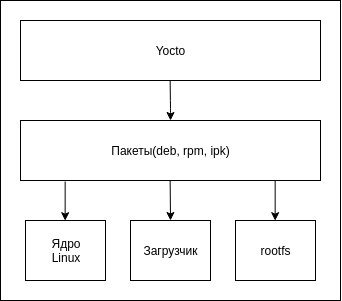
\includegraphics[height=8cm]{build/images/yocto}
  \caption{В yocto все части образа являются пакетами}\label{fig: yocto}
\end{figure}

Проект Yocto широко используется в отрасли и имеет поддержку многих влиятельных компаний. Кроме того, у этого есть большое и энергичное сообщество разработчиков и экосистема, способствующая этому. Сочетание энтузиастов с открытым исходным кодом и корпоративных спонсоров помогает вести проект\cite{YOCTO}.

\textbf{Преимущества использования Yocto:}
\begin{itemize}
  \item Проект легко расширяется через \textbf{слои}, которые можно публиковать независимо для добавления дополнительных функций или для хранения настроек, уникальных для целевой системы.
  \item Широкая поддержка со стороны многих производителей полупроводников и плат.
  \item Настройки для отдельного приложения могут храниться в слое для инкапсуляции и изоляции. Настройки, уникальные для слоя, как правило, хранятся как часть самого слоя, что позволяет применять одни и те же настройки одновременно к нескольким системным конфигурациям. 
  \item Yocto также предоставляет четко определенный уровень приоритета задач и возможность их переопределения. Это позволяет определить порядок применения слоев и поиска метаданных. Это также позволяет переопределить настройки в слоях с более высоким приоритетом.

\textbf{Недостатки использования Yocto:}
\end{itemize}
\begin{itemize}
  \item Время сборки и ресурсы разработки достаточно высоки\cite{YOCTO}. Так как количество пакетов, которые необходимо собрать, является значительным, а сборка происходит в несколько потоков. Рабочие станции для разработчиков Yocto, как правило, представляют собой большие системы. Однако, в Yocto имеется встроенный механизм кэширования, который позволяет повторно использовать ранее созданные компоненты, когда параметры для создания определенного пакета не изменились.
\end{itemize}
\newpage
\subsubsection{Buildroot}
Проект Buildroot это «простой, эффективный и простой в использовании инструмент для генерации встроенных систем Linux посредством кросс-компиляции»\cite{BUILDROOT}. 
Он разделяет многие из тех же целей, что и проект Yocto, однако он сфокусирован на простоте использования. 
По умолчанию Buildroot отключит все необязательные настройки времени компиляции для всех пакетов, что приведет к созданию образа с минимальным объемом. 
Разработчик системы должен будет включить настройки, необходимые для его встроенной системы.

Buildroot собирает все компоненты из исходного кода, но не поддерживает управление пакетами. Нет механизма для установки новых пакетов в работающую систему.
Результат сборки в целом состоит из трех компонентов:
\begin{itemize}
  \item \textbf{Основные модули} -- ядро, загрузчик и модули ядра, соответствующие целевому оборудованию(рис.~\ref{fig:buildroot}).;
  \item \textbf{rootfs} -- образ корневой файловой системы и любые другие вспомогательные файлы, необходимые для развертывания Linux на целевой платформе;
  \item \textbf{Набор инструментов,} которые использовалась для сборки всех целевых двоичных файлов;
\end{itemize}

\begin{figure}[h!]
  \centering
  \setlength{\fboxsep}{5pt}
  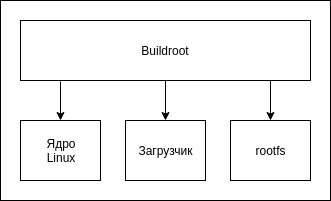
\includegraphics[height=8cm]{build/images/buildroot}
  \caption{В buildroot основные части образа поставляются вне пакетов}\label{fig:buildroot}
\end{figure}

\textbf{Преимущества использования Buildroot:}
\begin{itemize}
  \item Базовая система сборки написана на Make\cite{BUILDROOT} и достаточно коротка, чтобы позволить разработчику понять всю систему, в то же время будучи достаточно расширяемой для удовлетворения потребностей разработчиков встраиваемых Linux-систем;
Ядро Buildroot обычно обрабатывает только общие случаи использования, но его можно расширять с помощью сценариев;
  \item Система Buildroot использует для своей конфигурации Makefile и язык Kconfig\cite{BUILDROOT}. Kconfig был разработан сообществом разработчиков ядра Linux\cite{KCONFIG} и широко используется в проектах с открытым исходным кодом, что делает его знакомым для многих разработчиков;
  \item В связи со способом сборки, заключающейся в отключении всех необязательных настроек для каждого отдельного пакета, Buildroot обычно создает наименьшие по объему возможные образы с использованием готовой конфигурации. 
Время сборки и сборки ресурсов хоста в целом также будет меньше, чем с использованием Yocto;
\end{itemize}

\textbf{Недостатки использования Buildroot:}
\begin{itemize}
  \item Акцент на простоте и минимальных включенных параметрах сборки подразумевает, что разработчику может потребоваться выполнить объемную настройку сборки для пакета, если используется нестандартная конфигурация. Кроме того, все параметры конфигурации для пакета хранятся в одном файле\cite{BUILDROOT}, а это означает, что если проект поддерживает несколько аппаратных платформ, разработчику нужно будет вносить изменения в каждую настройку для каждой платформы;
  \item Любое изменение в файле конфигурации системы требует полной пересборки всех пакетов;
\end{itemize}

\newpage
\subsubsection{Системы адаптации дистрибутивов}
Распространенный подход к проектированию встраиваемых систем на основе Linux заключается в том, чтобы начать с настольного дистрибутива, такого как Debian или Red Hat, и удалять ненужные компоненты, пока установленный образ не поместится в пространство целевого устройства\cite{ARMBIAN}. Это подход, принятый для популярного дистрибутива Raspbian для платформы Raspberry Pi.

\textbf{Преимущества использования cистемы адаптации дистрибутивов:}
\begin{itemize}
  \item Основным преимуществом этого подхода является ознакомленность разработчика с содержимым дистрибутива. 
Часто разработчики встраиваемых Linux-систем также являются пользователями настольных Linux-систем и хорошо разбираются в своем дистрибутиве. 
Использование аналогичной среды на цели может позволить разработчикам начать работу быстрее.
В зависимости от выбранного дистрибутива, многие дополнительные инструменты могут быть установлены с использованием стандартных пакетных менеджеров, таких как apt и yum;
  \item Количество пакетов в репозиториях пакетных менеджеров, большинства настольных дистрибутивов, обычно больше, чем рецептов для Yocto или Buildroot;
  \item Благодаря встроенному менеджеру пакетов, такой дистрибутив удобно использовать во время разработки продукта в качестве отладочного окружения;
\end{itemize}

\textbf{Недостатки использования cистемы адаптации дистрибутивов:}
\begin{itemize}
  \item Получить воспроизводимую среду таким способом сложно так как поставщики пакетов могут обновлять их версии;
  \item Добавление и удаление пакетов вручную подвержено ошибкам;
\end{itemize}

\newpage
\subsection{Постановка задач исследования}
В рамках данной работы требуется спроектировать и реализовать программное обеспечение для сборки дистрибутивов операционных систем на основе Linux для встроенных систем.

Для достижения поставленной цели необходимо решить следующие задачи:
\begin{itemize}
  \item определить требования к системе;
  \item спроектировать архитектуру системы;
  \item реализовать программное обеспечение системы в соответствии с разработанной архитектурой;
  \item провести тестирование и апробацию;
\end{itemize}
\newpage

  % \input{src/2-design}
  % \mysection{ОПИСАНИЕ РЕАЛИЗАЦИИ ПРОГРАММНОГО ОБЕСПЕЧЕНИЯ}
\newpage

  % \mysection{ТЕСТИРОВАНИЕ И АПРОБАЦИЯ РАЗРАБОТАННОЙ СИТЕМЫ}
\newpage

  % \mysection*{ЗАКЛЮЧЕНИЕ}

В рамках проведённой работы были получены следующие результаты:
\begin{dashitemize}
  \item Проведен обзор и сравнение существующих систем сборки Linux дистрибутивов для встроенных сиетем.
  \item Создана архитектура системы, на основе которой было разработана система сборки, полностью удовлетворяющяя всем заявленным требованиям.
  \item Проведено функциональное тестирование системы сборки.
  \item Проведена апробация результатов работы. Система сборки была протестированы сотрудниками компании Emlid.
  \item На основе полученных в~ходе апробации отчётов об ошибках и~пожеланий произведены доработки системы. Разработанный продукт был успешно внедрён в~качестве системы сборки debian дистрибутивов для устройств Neutis N5.
\end{dashitemize}

Автор планирует продолжать работу над проектом и~развивать его, добавляя новые функции и~исправляя возможные ошибки, которые могут быть найдены во время эксплуатации системы.

\newpage

  % \input{src/6-definitions}

  \phantomsection
  \addcontentsline{toc}{section}{Библиографический список}

  \hyphenpenalty=10000
  \interlinepenalty=10000

  \nocite{*}
  \bibliography{biblio}
  
  \clearpage
  
  %\begin{appendices}
    %\input{src/appendices/events_module_listing}
    %\input{src/appendices/toggle_tests_listing}
  %\end{appendices}
\end{document}
